\begin{savequote}[75mm] 
If I have seen further it is by standing on the shoulders of giants
\qauthor{Isaac Newton} 
\end{savequote}

\chapter{Introduction}

\newthought{Bioinformatics is in its very nature multi--disciplinary}: biotechnology methods are used to capture the data, mathematical and statistical models are necessary to make sense of it; and software/hardware it is necessary to process all the information and everything should be seen under the prisma of the existing biological knowledge.

Techniques and methods trying to uncover the logic behind cellular proceses are in constant development. The success of such methods is usually related to the ability of isolating a particular state/measurement of the organic material (e.g. level of expression of a single protein, number of mutations of a gene in a population, etc.). However,  cellular functions of a higher level and organism's processes can only be study with a more holistic approach.

Integrating information from different experiments in context with the current knowledge-base is one of the most recurrent duties that researchers have to accomplish, this task however takes another dimension when the goal is aimed to a generic scope, and the strategy to connect related data sets should work in similar scenarios.

The challenges of integrate data in a more generic scope go from technical (e.g. incompatibilities of the storage systems) to structural (e.g. two datasets can refer to the same entity using different identifiers), but in overall the major challenge is to not lose the meaning on the connection (e.g. linking proteins and genes and knowing what is their relationship).

Integration of data usually refers to connecting data in low level, by means of storing aggregated information from several sources or by saving links to where the source is. However it is also possible to integrate on a higher level, where information is not saved and the aggregates are built on the fly and visualised in order to provide a wider view.

This project explores both, Integration and visualisation of information in bioinformatics; the rest of this introduction presents the state of the art and base technologies in both fields. Chapter 2 presents the efforts executed during this doctorate that contribute to the ways data is integrated in bioinformatics projects. Chapter 3 describes our inputs to the visualisation of data in bioinformatic, focusing in particular in a web tool for the visualisation of protein-protein interactions. The final chapter contains the conclusions of the project.


\section{Integration of information}
\subsection{State of the art}
The approaches to integrate data in bioinformatics are themselves heterogenous and focused on different types of integration, from simply linking resources to development of complex structures of aggregated information. In \cite{GOB2008} the authors categorise the different techniques used to integrate data in bioinformatics into 8 approaches, and then this categories were reorganised in \cite{ZHA2011b} into:
\begin{description}
\item[Data warehousing:] 			A centralised repository were the information from different sources is copied and processed to be kept  in a single place. providing a single access point to their data. However the preprocessing of the data is usually a complex process and the posterior additions or editions require lots of work.
\item[Federated databasing:] 		Multiple sources agree to follow a similar structure in order to allow an standard query over several instances. By dealing with smaller datasets than the data warehousing approach the complexity of post-processing is simplified, however it requires that the providers deal with the extra work of maintaining their data as the federated database agreement stablished.
\item[Service oriente integration:] 	Definition of a protocol for requests and responses to obtain data or execute services. The 2 standards widely used are SOAP (Simple Object Access Protocol) services and REST (REpresentational State Transfer) services, where the latter is getting momentum because of its simplicity. However this also requires big commitment from providers about creating and maintaining the services, and also increasing and maintaining the specifications fro the different domains.
\item[Semantic integration:] 		Structure the data using semantic web standards(e.g. RDF, OWL) in order to make it ``machine-readable'' and be able to deduce meaningful associations. The conversion of the data into RDF files might not be a trivial work, and it has similar problems to the one mentioned above because it maintains copies of the information in a separate format, 
\item[Wiki-based integration:] 		Cooperative effort where the community inputs information in a open and unstructured way, which can reach a highly reliable status as has been shown by the wikipedia case, but is completely dependent on the adoption of the community, and also given the unstructured nature of the data is hard to manipulate for automatic analysis.
\end{description}

we now present some of the most representative projects that have attempted to integrate data and offer a solution for this need in the bioinformatics field, by using one or more of the mentioned approaches. 

%\section{Current Projects for Data Integration in Bioinformatics}
\subsubsection{Atlas}
info
\subsubsection{BioMart}
\subsubsection{SRS}
\subsubsection{BioMOBY}
\subsubsection{Taverna and Galaxy}
\subsubsection{Bio2RDF}
\subsubsection{WikiGenes and WikiProteins}

\subsection{The Distributed Annotation System}
The Distributed Annotation System (DAS) is... \cite{JEN2008} and I can use Fig.~\ref{fig:das}. to explain:
\begin{figure}  
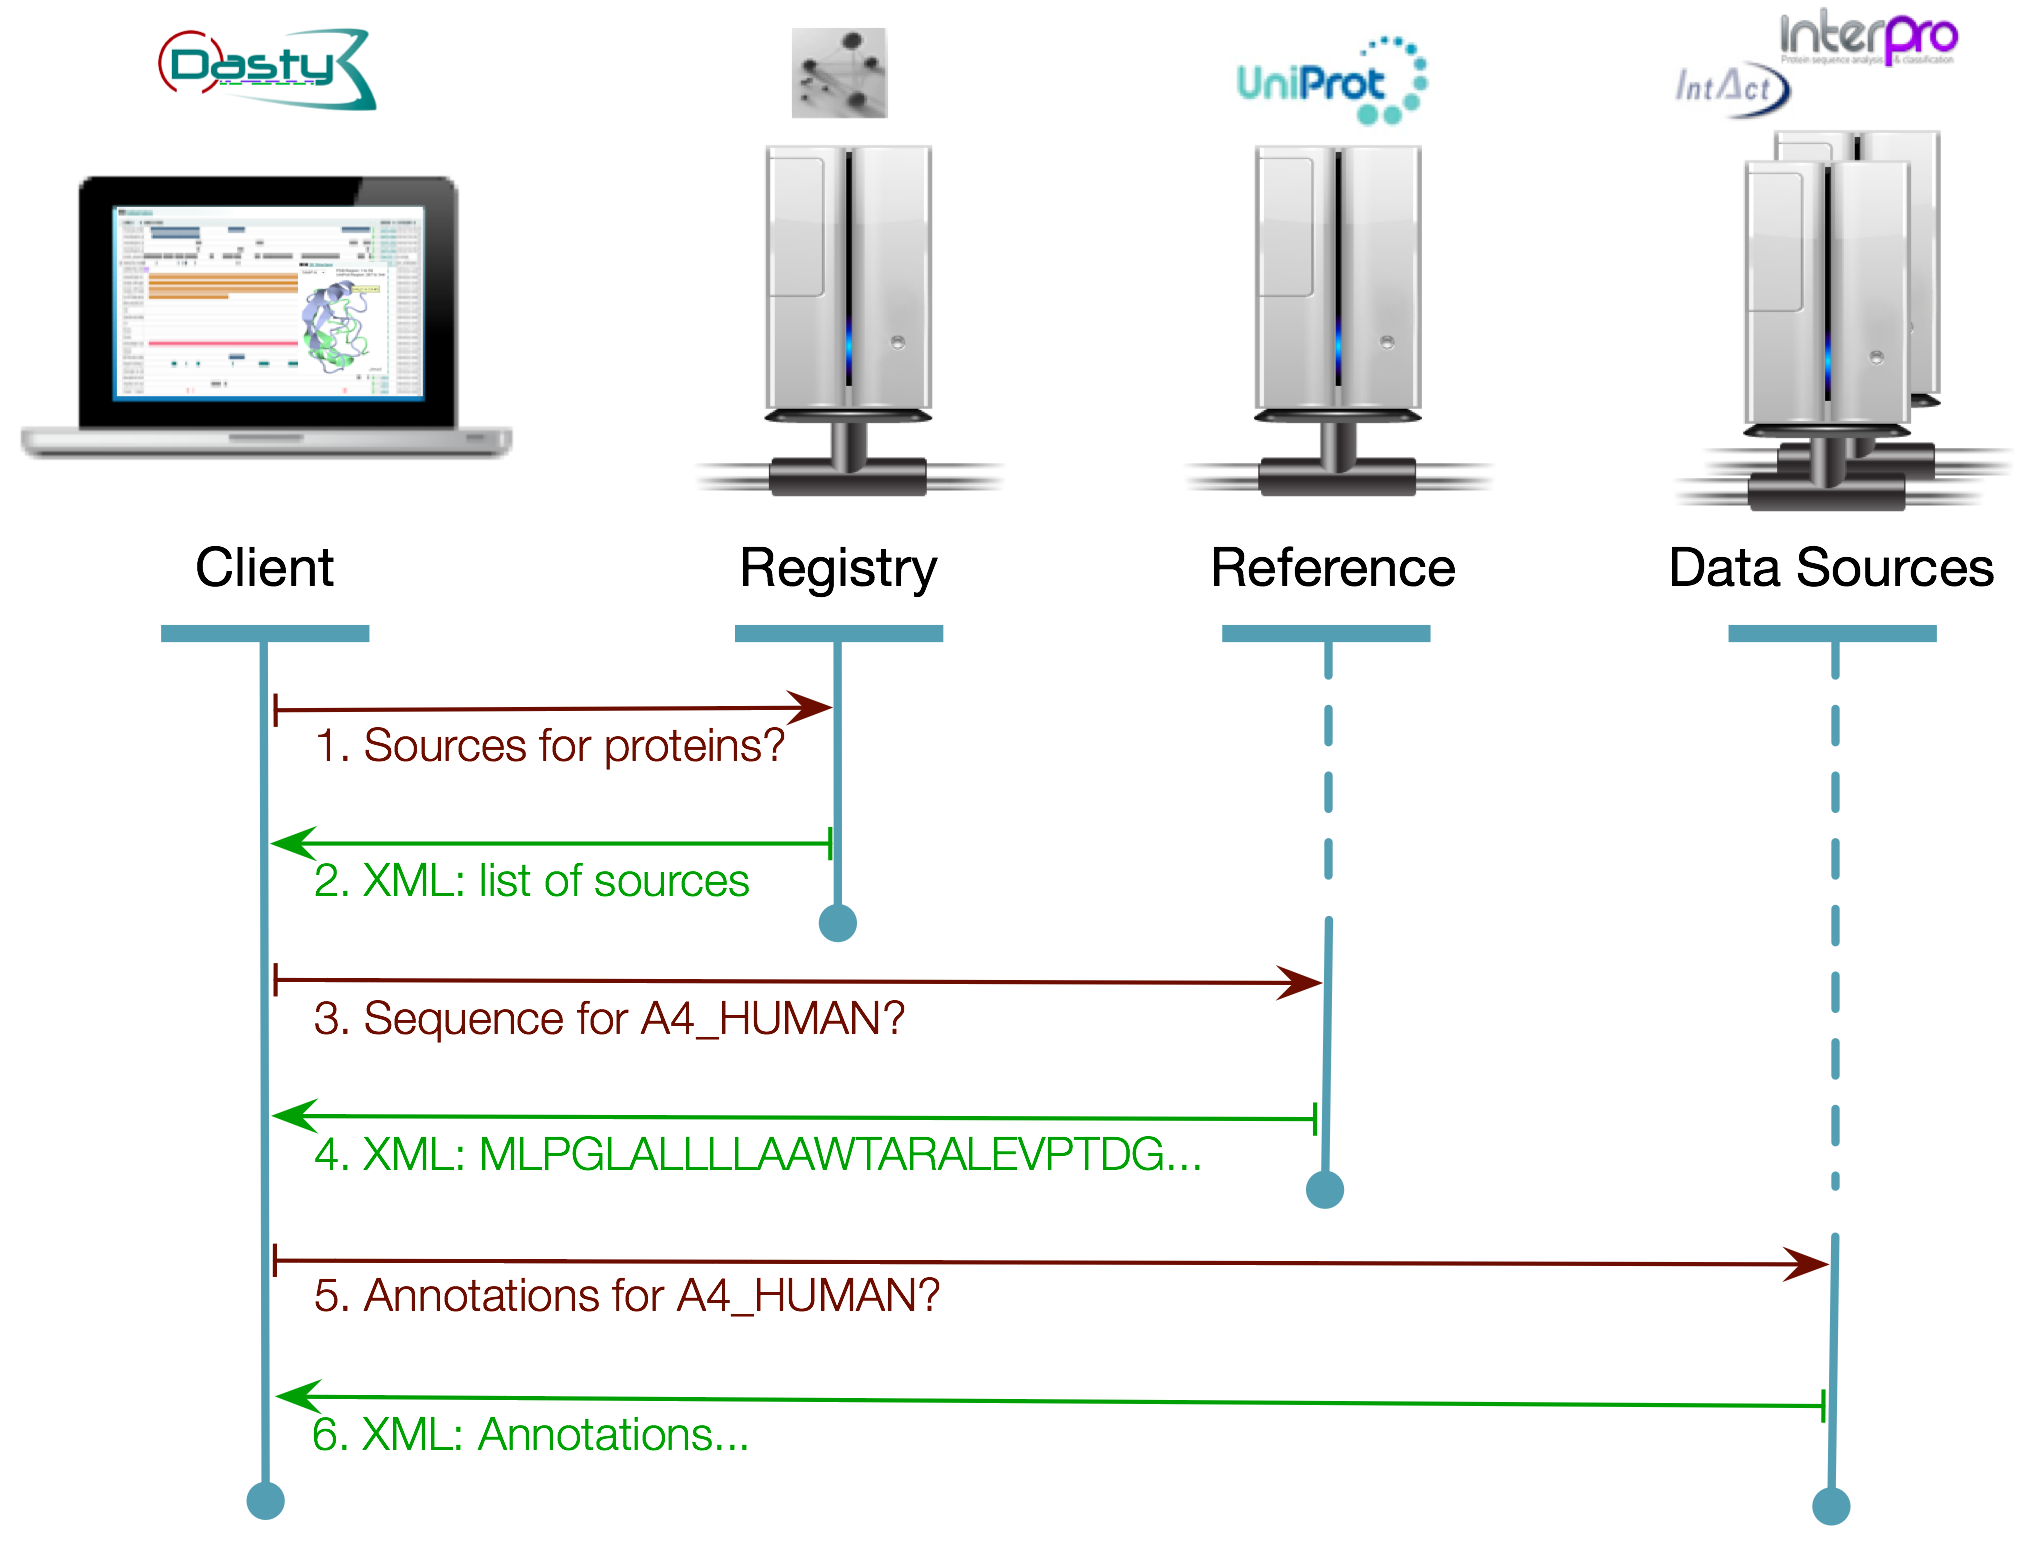
\includegraphics[width=\textwidth]{figures/DAS.png}
\caption[DAS Flow of Information.]{Flow of information in a standard query in the Distributed Annotating System.
\label{fig:das}}
\end{figure}
we should describe Dasty3 \cite{VIL2011}

\begin{savequote}[75mm] 
Our posturings, our imagined self-importance, the delusion that we have some privileged position in the Universe, are challenged by this point of pale light.
\qauthor{Carl Sagan, Pale Blue Dot, 1994} 
\end{savequote}
\section{Visualization}
The field of visualization aims to represent data in a way that non evident features became visible. The developed techniques in this search varies from simple ones (e.g. histograms) to very elaborated (e.g. environments just visible using 3D virtual reality rooms).

The uses of visualization techniques are as diverse as fields are in the world, from weather forecast in the news to the analysis of the captured data in the Large Hadron Collider. In the field of our interest: bioinformatics, the use of visualization methods is also abundant and sub-fields such as genomics, proteomics, population variance, etc. have plenty of examples were different techniques have been implemented with the purpose of making sense of biological data via visual representations.

The section below is a review of the most relevant existing tools in different bioinformatics fields.
\subsection{Visualization tools in Bioinformatics}
Small intro for the subsection
\subsubsection{Genomics}
Ensembl, mykarioView, Dalliance, IGV, Tablet, BAMView
\subsubsection{Proteomics}
Dasty, Interpro
\subsubsection{Protein Interaction}
\subsubsection{Population Variation}
\subsubsection{General Research}
To talk about statistical graphs and things like heat maps, phylogenetic trees, etc.


\section{Thesis outline}
